\begin{frame}{Est-on d'accord?}
  {}{\scriptsize
    Instructions:
    \begin{enumerate}
      \item<2-> Un/e étudiant/e pose une question en indiquant les objets dans l'image
      \item<3-> Un/e autre étudiant/e donne la réponse en utilisant un nombre et le nom des objets
      \item<4-> Un/e autre étudiant/e dis si on est d'accord ou non en utilisant un nombre et le pronom \lexi{en}
    \end{enumerate}
  }
  \begin{columns}
    \column{0.4\textwidth}
      \begin{itemize}
        \item[E1:] Il y a combien de \underline{\uncover<2-4>{boîtes de pizza}}?
        \item[E2:] Il y a \underline{\uncover<3-4>{trois boîtes de pizza}}.
        \item[E3:] \underline{\uncover<4>{Non}}, il y en a \underline{\uncover<4>{quatre}}.
      \end{itemize}
    \column{0.6\textwidth}
      \begin{minipage}[c][0.6\textheight]{\linewidth}
        \begin{center}
          \only<-4>{
            
\includegraphics[scale=0.25]{pizza_boxes.jpg}
          }
          \only<5>{
            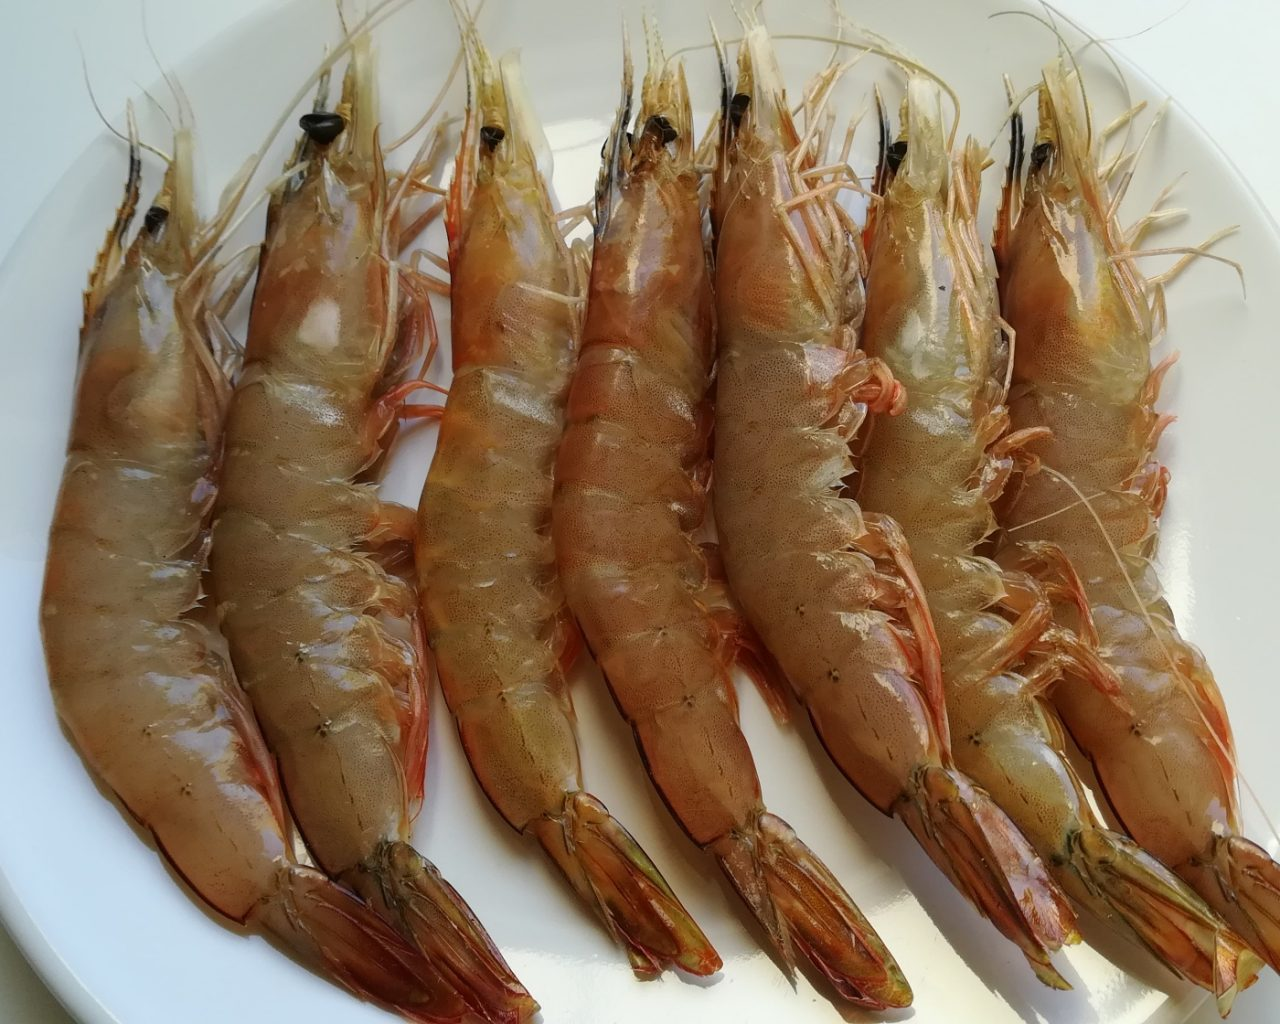
\includegraphics[scale=0.15]{crevettes.jpg}
          }
          \only<6>{
            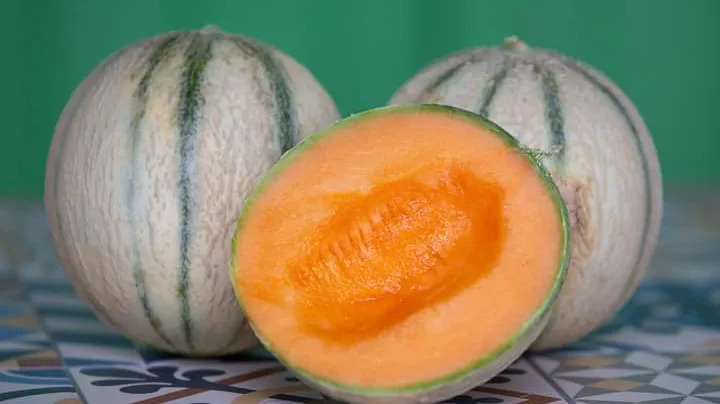
\includegraphics[scale=0.28]{melons.jpg}
          }
          \only<7>{
            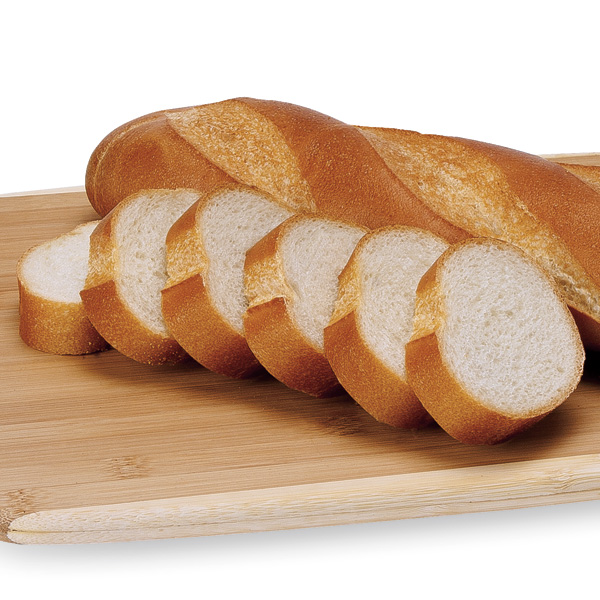
\includegraphics{tranches.jpg}
          }
          \only<8>{
            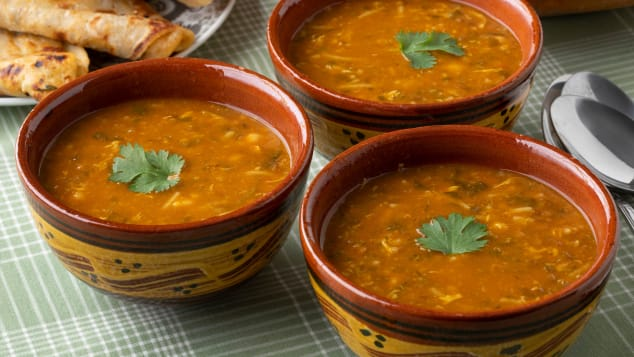
\includegraphics[scale=0.33]{bols.jpg}
          }
          \only<9>{
            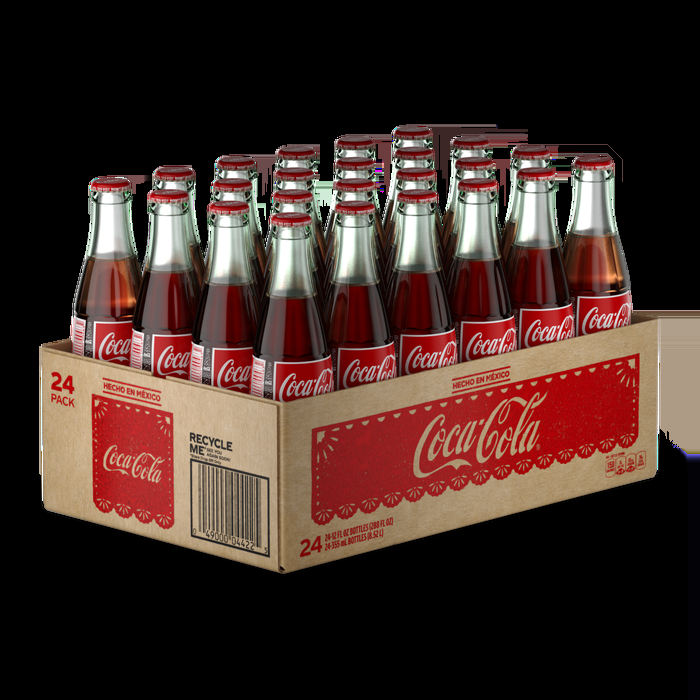
\includegraphics[scale=0.2]{bouteilles.jpg}
          }
        \end{center}
      \end{minipage}
  \end{columns}
\end{frame}